\documentclass[UTF8,10pt,a4paper,fontset=fandol]{ctexart}

\usepackage[a4paper,top=10mm,bottom=10mm,left=11.5mm,right=11.5mm]{geometry}
\usepackage{graphicx}
\usepackage{xcolor}
\usepackage{microtype}
\usepackage{hyperref}
\usepackage{enumitem}
\usepackage{tabularx}
\usepackage{array}
\usepackage{ragged2e}
\usepackage{setspace}
\usepackage{calc}
\renewcommand{\familydefault}{\sfdefault}
\renewcommand{\CJKfamilydefault}{\CJKsfdefault}
\graphicspath{{../public/}{./}}

\definecolor{Navy}{HTML}{17324D}
\definecolor{Teal}{HTML}{0F7182}
\definecolor{Ink}{HTML}{17202A}
\definecolor{Muted}{HTML}{5D6773}
\definecolor{Rule}{HTML}{D6DEE5}
\definecolor{Soft}{HTML}{EEF4F7}
\definecolor{SoftBlue}{HTML}{E7F1F4}

\hypersetup{
  colorlinks=true,
  urlcolor=Teal,
  linkcolor=Navy,
  pdfauthor={纪家灏 Jia-Hao Ji},
  pdftitle={纪家灏 - 中文一页研究简历},
  pdfsubject={生物医学人工智能、空间组学与多智能体推理},
  pdfkeywords={人工智能, 医学, 空间组学, 多智能体系统, 神经科学}
}
\urlstyle{same}

\pagestyle{empty}
\setlength{\parindent}{0pt}
\setlength{\parskip}{0pt}
\setstretch{1.00}
\emergencystretch=1em
\hyphenpenalty=10000
\exhyphenpenalty=10000

\newcommand{\sectiontitle}[1]{%
  \vspace{0.46em}%
  {\fontsize{10.5}{11.4}\selectfont\bfseries\color{Navy}#1}\par
  \vspace{-0.22em}\color{Rule}\rule{\linewidth}{0.45pt}\color{Ink}\vspace{0.24em}
}
\newcommand{\sideheading}[1]{%
  \vspace{0.38em}%
  {\fontsize{9.2}{10}\selectfont\bfseries\color{Navy}#1}\par
  \vspace{0.10em}\color{Teal}\rule{\linewidth}{0.7pt}\color{Ink}\vspace{0.22em}
}
\newcommand{\smallmeta}[1]{{\fontsize{7.55}{8.95}\selectfont\color{Muted}#1}}
\newcommand{\bodytext}[1]{{\fontsize{8.0}{9.55}\selectfont\RaggedRight #1}}
\newcommand{\pubentry}[4]{%
  {\fontsize{8.55}{9.9}\selectfont\bfseries\color{Ink}\RaggedRight #1}\par
  \smallmeta{#2}\par
  \vspace{0.05em}
  {\fontsize{7.85}{9.25}\selectfont\RaggedRight #3}\par
  \vspace{0.04em}
  {\fontsize{7.55}{8.9}\selectfont\bfseries\color{Teal}#4}\par
  \vspace{0.30em}
}
\newcommand{\role}[3]{%
  \begin{tabularx}{\linewidth}{@{}>{\RaggedRight\arraybackslash}X>{\RaggedLeft\arraybackslash}p{23mm}@{}}
    {\fontsize{8.35}{9.6}\selectfont\bfseries\color{Ink}#1} & {\fontsize{7.45}{8.7}\selectfont\color{Muted}#3}\\[-0.08em]
    {\fontsize{7.8}{9.0}\selectfont\color{Teal}#2} &
  \end{tabularx}\vspace{0.02em}
}
\newenvironment{compactitems}{%
  \begin{itemize}[leftmargin=1.05em,itemsep=0.06em,topsep=0.06em,parsep=0pt,partopsep=0pt,label=\textcolor{Teal}{\raisebox{0.18ex}{\tiny\textbullet}}]
  \fontsize{7.75}{9.15}\selectfont\RaggedRight
}{\end{itemize}}
\newcommand{\sidebaritem}[2]{%
  {\fontsize{7.95}{9.15}\selectfont\bfseries\color{Ink}\RaggedRight #1}\par
  {\fontsize{7.45}{8.8}\selectfont\color{Muted}\RaggedRight #2}\par\vspace{0.26em}
}
\newcommand{\skillline}[2]{%
  {\fontsize{7.7}{8.95}\selectfont\bfseries\color{Navy}\RaggedRight #1}\par
  {\fontsize{7.35}{8.75}\selectfont\color{Ink}\RaggedRight #2}\par\vspace{0.23em}
}
\newcommand{\tag}[1]{\colorbox{SoftBlue}{\strut\hspace{0.26em}\fontsize{7.0}{8.1}\selectfont\bfseries\color{Navy}#1\hspace{0.26em}}}

\begin{document}
\fontsize{8.0}{9.5}\selectfont

% Header
\begin{tabularx}{\textwidth}{@{}X>{\RaggedLeft\arraybackslash}p{31mm}@{}}
  \begin{minipage}[t]{\linewidth}
    \vspace{0pt}
    {\fontsize{24}{26}\selectfont\bfseries\color{Ink}纪家灏}\par
    \vspace{0.06em}
    {\fontsize{10.2}{11.4}\selectfont\bfseries\color{Navy}Jia-Hao (Jay) Ji}\par
    \vspace{0.18em}
    {\fontsize{10.8}{12.0}\selectfont\bfseries\color{Navy}复旦八年制临床医学在读｜人工智能研究者}\par
    \vspace{0.34em}
    {\fontsize{8.15}{9.55}\selectfont\color{Muted}\RaggedRight
      研究生物医学人工智能、空间组学和多智能体推理，重点开发可追溯、可评价的科研智能体与多模态分析系统。
    }\par
    \vspace{0.34em}
    {\fontsize{7.45}{8.7}\selectfont\color{Muted}
      上海 \hspace{0.35em}\textcolor{Rule}{\textbullet}\hspace{0.35em}
      \href{mailto:jhji19@fudan.edu.cn}{jhji19@fudan.edu.cn} \hspace{0.35em}\textcolor{Rule}{\textbullet}\hspace{0.35em}
      \href{https://jiahaoblog.com/about/zh/}{中文主页} \hspace{0.35em}\textcolor{Rule}{\textbullet}\hspace{0.35em}
      \href{https://github.com/Biogod2020}{GitHub} \hspace{0.35em}\textcolor{Rule}{\textbullet}\hspace{0.35em}
      \href{https://orcid.org/0009-0007-4647-522X}{ORCID}
    }\par
  \end{minipage}
  &
  \begin{minipage}[t]{31mm}
    \vspace{0pt}
    \fcolorbox{Rule}{white}{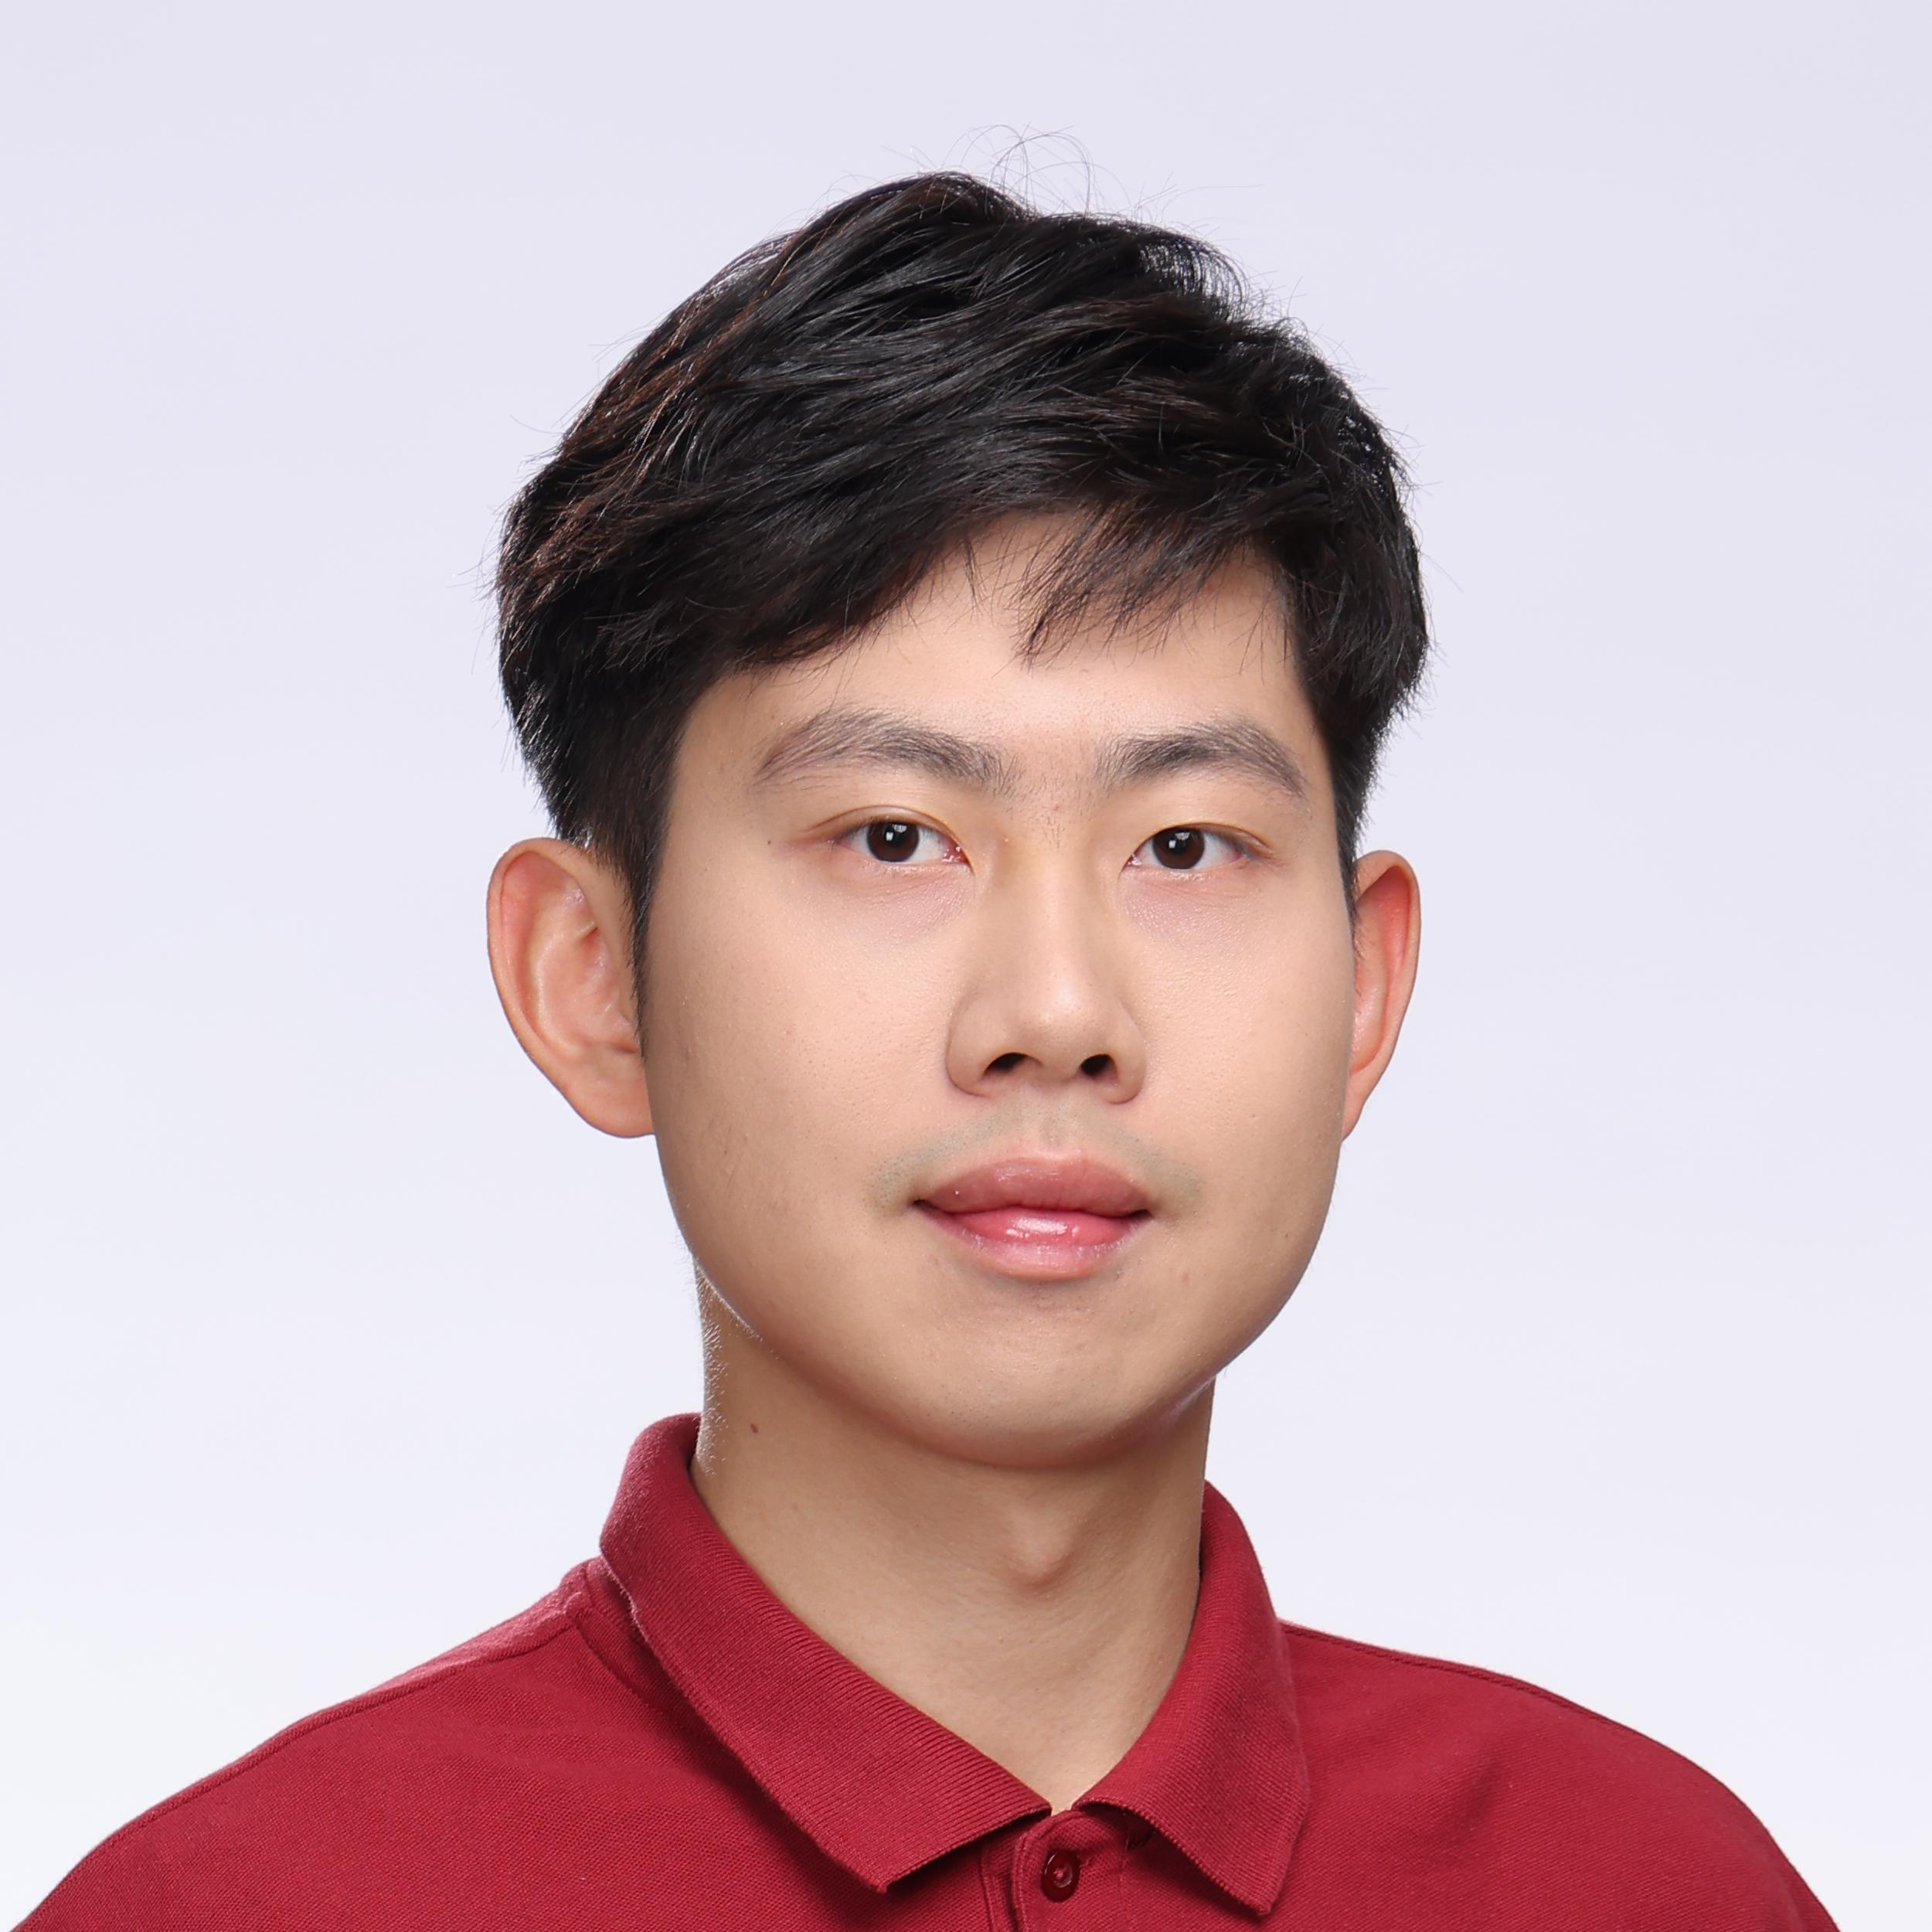
\includegraphics[width=27.5mm,trim=460 465 460 60,clip]{avatar.jpg}}
  \end{minipage}
\end{tabularx}

\vspace{0.32em}
\color{Navy}\rule{\textwidth}{1.7pt}\color{Ink}
\vspace{0.31em}

\tag{科学智能体}\hspace{0.30em}
\tag{空间组学}\hspace{0.30em}
\tag{多模态学习}\hspace{0.30em}
\tag{多智能体推理}\hspace{0.30em}
\tag{神经科学}

\vspace{0.12em}

% Two-column body
\begin{minipage}[t]{0.665\textwidth}
\vspace{0pt}\RaggedRight

\sectiontitle{代表性研究}

\pubentry
{候选答案供给与最终选择共同决定大模型评审在多智能体系统中的价值}
{\textbf{纪家灏}等，第一作者，arXiv:2608.25937，2026。\href{https://arxiv.org/abs/2608.25937}{论文}}
{把多智能体推理拆分为候选生成、答案识别与终端选择。五个基准中，正确答案经常已进入候选池，系统仍会在最终环节选错。}
{15,336 个问题｜81,390 次固定候选池回放｜仅改变选择规则，准确率由 63.82\% 提升至 70.82--70.95\%}

\pubentry
{SpatialDataAgent：十年尺度空间组学数据的自主整理}
{\textbf{纪家灏}等，第一作者兼主要开发者，bioRxiv，2026。\href{https://doi.org/10.64898/2026.05.27.727615}{DOI}}
{负责总体设计与主要开发，建立可追溯的智能体工作流，完成空间组学记录的检索、证据核验和标准化。}
{769 组 H\&E--空间转录组配对数据｜2,920 万个空间点或细胞｜覆盖规模达到既有人工整理基线的 6.4 倍}

\pubentry
{时空转录组揭示与阿尔茨海默病胆碱能易损性相关的反应性基底前脑小胶质细胞}
{\textbf{纪家灏}（共同第一作者）等，\textit{Cell} 审稿中，2026。}
{共同第一作者。整合空间转录组、单核测序与原位淀粉样病理，分析小胶质细胞状态与胆碱能神经元易损性的关系。}
{1,236 万个空间表达谱}

\sectiontitle{科研经历}

\role{科研项目负责人}{复旦大学数据驱动未来创新实验室｜医学遗传研究院}{2023.09--至今}
\smallmeta{导师：郁金泰教授、原致远教授｜阿尔茨海默病、空间组学与生物医学人工智能}
\begin{compactitems}
  \item 负责大规模空间数据整理、多模态组织配准，以及组织学与分子表达联合分析。
  \item 开发 Transformer 与图像配准方法，对齐全切片病理图像和空间转录组坐标；构建带有结构化输出约束、证据追踪和多阶段验证的智能体流程。
  \item 使用固定候选池回放实验评估大模型评审可靠性与终端答案选择。
\end{compactitems}

\vspace{0.12em}
\role{本科科研成员}{复旦大学宋彬教授课题组}{2021.10--2023.06}
\begin{compactitems}
  \item 构建单细胞 RNA 测序分析流程，识别与 iPSC 来源多巴胺能前体细胞移植纯度、安全性及治疗潜力相关的分子标志物。
\end{compactitems}

\vspace{0.08em}
\role{本科科研成员}{复旦大学生物医学研究院｜蓝斐教授课题组}{2019.09--2021.07}
\begin{compactitems}
  \item 接受分子生物学、细胞培养、DNA 甲基化、表观遗传调控及基础生化实验训练。
\end{compactitems}

\sectiontitle{代表性系统}
\bodytext{\textbf{ASSA}：用于长程任务的模块化智能体框架，整合分层记忆、反思和技能生成（\href{https://github.com/Biogod2020/ASSA}{GitHub}）。\quad \textbf{Spatial-CLIP}：通过对比学习对齐组织病理图像和空间转录组状态（\href{https://github.com/Biogod2020/Spatial-Clip}{GitHub}）。}

\end{minipage}
\hfill
\color{Rule}\vrule width 0.45pt\color{Ink}
\hfill
\begin{minipage}[t]{0.295\textwidth}
\vspace{0pt}\RaggedRight

\sideheading{教育与临床训练}
\sidebaritem{复旦大学上海医学院}{八年制临床医学专业\\2019.09--2027.06（预计）}
\sidebaritem{加州大学洛杉矶分校}{国际交换项目\\2021.09--2022.02}
\sidebaritem{香港大学玛丽医院}{内科学系临床选修\\2025.04--2025.05}

\sideheading{研究方向}
\skillline{科学智能体}{开发可追溯、可评价的科研数据与工作流系统。}
\skillline{多模态生物医学 AI}{融合空间组学、数字病理和神经系统疾病研究。}
\skillline{可靠多智能体推理}{研究候选生成、大模型评审、通信和答案选择。}

\sideheading{技术能力}
\skillline{机器学习}{PyTorch、Transformer、图神经网络、对比学习、视觉语言模型、大模型智能体、多智能体系统。}
\skillline{生物医学数据}{空间转录组、单细胞 RNA 测序、全切片图像、组织病理、计算神经科学。}
\skillline{工程与计算}{Python、R、TypeScript、Linux、Git、高性能计算、多 GPU 训练、并行 API 工作流。}

\sideheading{教学与荣誉}
\bodytext{为复旦大学本科生和研究生讲授 AI 科研工作流，内容涵盖文献检索、科研写作和可复现研究，2025。}\par
\vspace{0.28em}
\bodytext{全国中学生生物学联赛一等奖，广东省第 9 名。}\par

\sideheading{语言}
\bodytext{普通话、粤语、潮州话；英语（TOEFL 105）；西班牙语（基础）。}

\vfill
{\fontsize{7.0}{8.1}\selectfont\color{Muted}更新于 2026 年 9 月}

\end{minipage}

\end{document}
